\documentclass[12pt]{article}
\usepackage{verbatim}
\usepackage[dvips]{epsfig}
\usepackage{color}
\usepackage{url}
\usepackage[colorlinks=true]{hyperref}

\begin{document}

\section*{GENESIS: Documentation}

{\bf Related Documentation:}
% start: userdocs-tag-replace-items related-do-nothing
% end: userdocs-tag-replace-items related-do-nothing

\section*{De Schutter: Purkinje Cell Model}

\begin{figure}[h]
\centering
   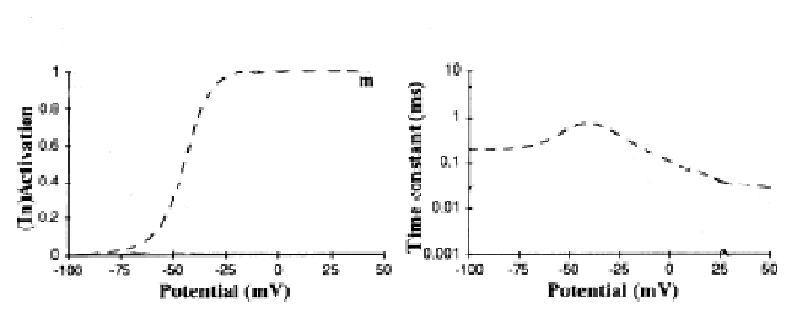
\includegraphics[scale=0.75]{figures/DS1.2Ap.eps}
   \caption{Activation properties of the persistent Na$^+$ (NaP, - - -, no inactivation) ionic conductance in the model. Seady-state activation vs. voltage are plotted at the {\em left} and the time constant of activation ($\tau_m$) vs. voltage on the {\em right} (Note: Semilogarithmic scale).}
   \label{fig:DS1.2Ap}
\end{figure}

\subsection*{Persistent Sodium Current}

The persistent sodium (NaP) current is assumed to cause the plateau potentials in the soma described by\,\cite{R:1980ly}. The basis for the equations describing NaP current were single-electrode voltage-clamp recordings of NaP current in guinea pig hippocampal neurons\,\cite{C-R-French:1990uq}. These recordings provided steady-state activation data and we assumed the same number of gates as for the NaF channel\,\cite{hodgkin52:_quantitative_description}. Time constants for activation and deactivation and the threshold of activation for NaP current were obtained from\,\cite{Kay:1990kx}. Note: The NaP current activation follows a slope similar to that of NaF current activation, but with a lower threshold of activation.

\bibliographystyle{plain}
\bibliography{../tex/bib/g3-refs}

\end{document}
